\documentclass[11pt, a4paper]{article}
\usepackage[utf8]{inputenc}
\usepackage{amsmath}
\usepackage{hyperref}
\usepackage{graphicx}
\usepackage{caption}
\usepackage{subcaption}

\graphicspath{{figures/}}

\title{\textbf{Models and Conventions for Universal Photonic Processors}}
\author{ Francesco Ceccarelli }
\date{\today}

\begin{document}
\maketitle

\section{Introduction}
This document aims at illustrating the software architecture and the conventions (physical, mathematical, and programming) adopted in the ``digital twin'' models for Universal Photonic Processors (UPP). In particular, it refers to the implementations contained in the \texttt{model.py} module, which defines objects simulating a photonic processor based on a sequence of mixing layers (directional couplers) and phase shifters. The software is capable of calculating multiple optical configurations in parallel, leveraging batch processing.

\section{Class Hierarchy}
The software architecture is based on an object-oriented approach that exploits inheritance to define common operations across different photonic network topologies, delegating specific implementations to derived models.

\begin{itemize}
    \item \textbf{\texttt{Mesh}}: This is the abstract base class that defines the standard interface and internal data structures shared by all processor topologies. It is not instantiated directly, but implements and manages common logic such as importing or generating hardware calibration and bidirectional translation between currents and optical phases.
    \item \textbf{\texttt{Clements}}: A subclass that implements the photonic processor topology based on the scheme by Clements et al. (Optica 3.12, 2016).
    \item \textbf{\texttt{Bell}}: A subclass that implements the architecture according to the scheme described by Bell et al. (APL Photonics 6.7, 2021).
\end{itemize}

\section{Attributes and Variables}
All photonic processor instances share fundamental attributes and adhere to precise physical and notational conventions, defined and initialized within the \texttt{Mesh} base class.

\subsection{Physical Modeling}
The phase reconfigurability is modeled through the following variables:
\begin{itemize}
    \item \textbf{Optical phases (\texttt{static\_phases} and \texttt{phases})}: Phases are strictly expressed in radians (\text{rad}) and constrained to the interval $[0, 2\pi)$ via modulo operations.
    \item \textbf{Actuation currents (\texttt{currents})}: The currents driving the thermo-optic phase shifters are expressed in milliamperes (\text{mA}).
    \item \textbf{Thermal cross-talk (\texttt{xtalk})}: The coefficients linking the square of the current to the induced phase is measured in $\text{rad}/\text{mA}^2$. 
\end{itemize}
Consequently, the calibration relationship (with cross-talk compensation) is based on matrix equations of the form:
\begin{equation}
    \texttt{phases} = \texttt{static\_phases} + \texttt{currents}^2 \times \texttt{xtalk}^T
\end{equation}
This relation cannot be inverted in general, as different current settings can yield the same phase configuration. Therefore, the solution minimizing power consumption must be found. We employ a heuristic method that, while not guaranteeing a global minimum, finds a valid solution that is optimal in most cases.
    
\subsection{Data Structure and Dimension}
Useful variables setting the dimension of the problem are:
\begin{itemize}
    \item \textbf{Optical modes (\texttt{n\_modes})}: This parameter defines the number of optical waveguides comprising the mesh. By current convention, the processor must have an even number of optical modes. If an odd number is provided as input, it is automatically decremented by one.
    \item \textbf{Available and used phases (\texttt{n\_phases} and \texttt{n\_used\_phases})}: A distinction is made between \texttt{n\_phases}, which is the total number of tunable parameters, and \texttt{n\_used\_phases}, which indicates the parameters actually utilized in the UPP:
        \begin{align}
        \texttt{n\_phases} &= \texttt{n\_modes} (\texttt{n\_modes} - 1) \\
        \texttt{n\_used\_phases} &= (\texttt{n\_modes} - 1)^2
    \end{align}
    Although \texttt{currents}, \texttt{phases} and \texttt{static\_phases} are vectors having shape (\texttt{n\_phases},) and \texttt{xtalk} is a matrix having shape \texttt{(n\_phases, n\_phases)}, some elements of these arrays are forced to zero via the boolean masks \texttt{static\_phases\_mask} and \texttt{xtalk\_mask}, respectively. In this way, we have vectors having only \texttt{n\_used\_phases} nonzero elements, while the matrix has a specific structure defined by the chosen topology (Clements or Bell). The specific structure of these arrays is detailed in Section \ref{sec:clements} and \ref{sec:bell}. The masks are useful not only for enforcing a given structure to the dataset, but also during the heuristic inversion (to calculate currents from target phases), when dimensions are reduced by extracting active rows and/or columns through boolean indexing to avoid mathematical singularities.
\end{itemize}
This parameter count directly relates to the expressivity of the photonic mesh and the reachable subspace of unitary matrices. Specifically, the required degrees of freedom scale as follows:
\begin{itemize}
    \item $\texttt{n\_modes}^2$ tunable parameters are required to span the full unitary group $U(N)$.
    \item $\texttt{n\_modes}(\texttt{n\_modes}-1)$ parameters can span $U(N)$ up to a single diagonal matrix of phase shifts (external output phases in our UPPs).
    \item $(\texttt{n\_modes}-1)^2$ parameters are sufficient to span $U(N)$ up to \textit{both} input and output diagonal matrices of phase shifts. By mathematically factoring out these external phases, the transformation can be reduced to a canonical \textit{real-bordered matrix} (where the elements of the first row and first column are strictly real). In many practical applications, such as those relying on intensity modulation and detection, these external phases are physically irrelevant, making this subset perfectly adequate for universal processing and for evaluating the actual operational fidelity.
\end{itemize}


\subsection{Tensor Notation}
Full tensor notation allows us to efficiently manage the multidimensional datasets:
\begin{itemize}
    \item \textbf{Mixing matrices and unitary representation}: Optical propagation through the photonic mesh is modeled using complex unitary matrices ($U$), calculated by multiplying a number \texttt{n\_mixing\_layers} of static mixing layers (\texttt{M}), based on directional couplers, alternated with phase shifts. Mixing layers and phase shifts depend on the topology (Clements or Bell), see Section \ref{sec:clements} and \ref{sec:bell} for a detailed discussion.
    \item \textbf{Batch processing}: The model supports and encourages parallel computing (\textit{batch processing}). Tensors representing currents and phases support both single-dimension shapes \texttt{(n\_phases,)} and vectorized shapes with a batch dimension \texttt{(B, n\_phases)}. Similarly, the resulting unitary matrices are handled with dimensions \texttt{(n\_modes, n\_modes)} or \texttt{(B, n\_modes, n\_modes)}.
\end{itemize}

\section{Clements Model}
\label{sec:clements}
Figure \ref{fig:clements_base} illustrates the waveguide and phase shifter topology for a Clements UPP. Each Mach-Zehnder interferometer (MZI) incorporates an internal phase shifter (depicted in red) to control the splitting ratio and an external phase shifter (in blue) for phase reconfiguration. The entire circuit can be viewed either as a mesh of MZI cells or, more conveniently from a computational perspective, as a cascade of alternating mixing and phase layers. While the mixing layers are shared between both the Clements and Bell architectures, the phase shifter arrangement differs; consequently, \texttt{U\_from\_phases} and \texttt{phases\_from\_U} are methods dependent on the specific architecture and are therefore implemented directly within the respective derived classes. Finally, Figure \ref{fig:clements_base} also details the phase shifter numbering scheme utilized in the software implementation.
\begin{figure}[htbp]
    \centering
    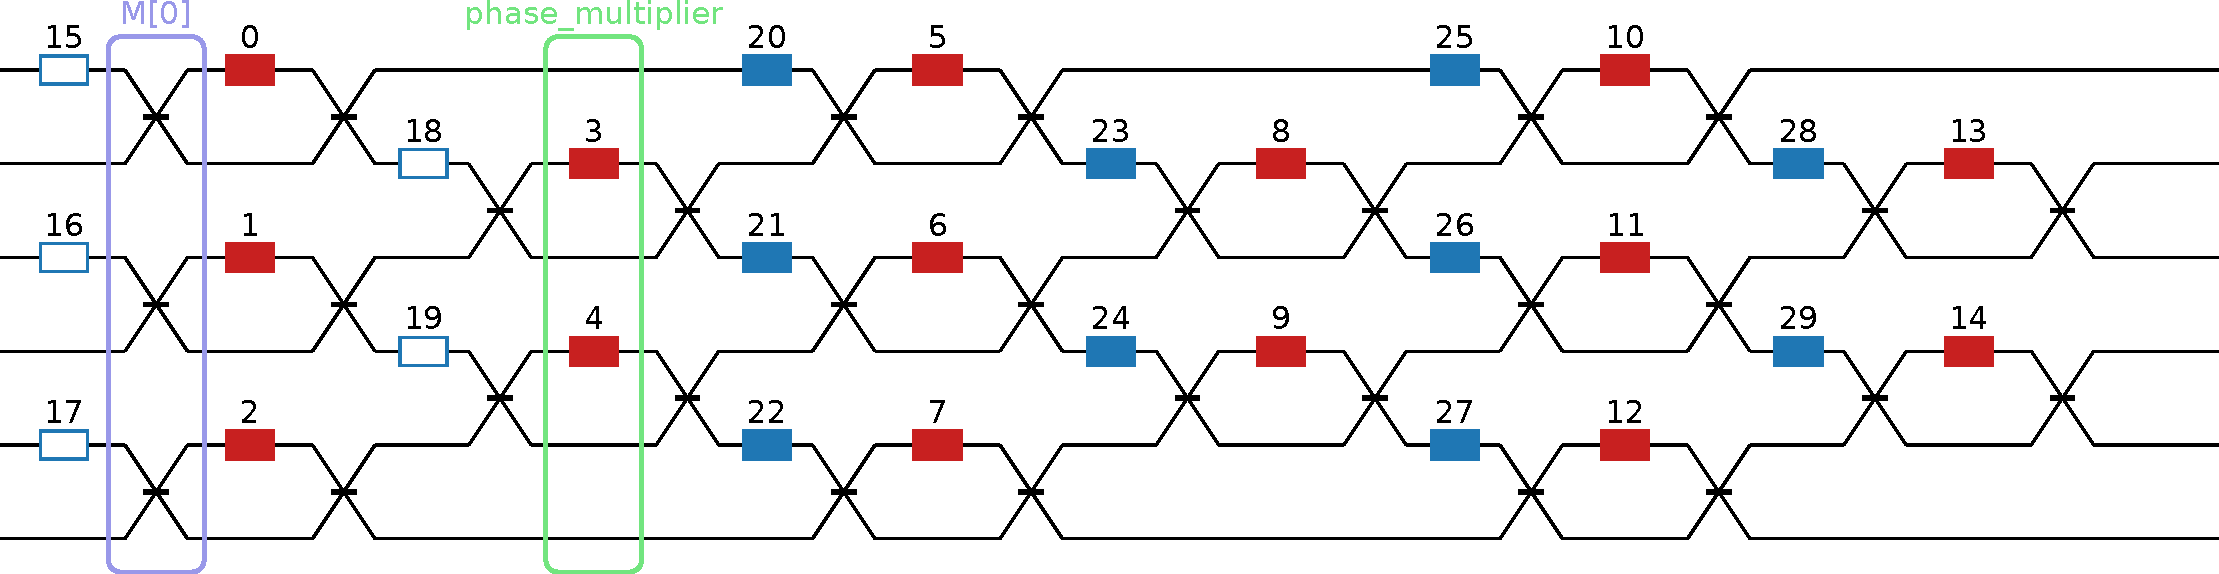
\includegraphics[width=\textwidth]{clements_base.pdf}
    \caption{Topology and numbering scheme for a 6-mode Clements processor. We highlight the first mixing layer \texttt{M[0]} and the \texttt{phase\_multiplier} variable corresponding to iteration 3.}
    \label{fig:clements_base}
\end{figure}

\subsection{Used Phases}
Figure \ref{fig:clements_base} illustrates the phase shifters actively used (depicted as solid) for circuit operation versus those considered redundant (hollow ones). This directly affects the structure of the \texttt{phases}, \texttt{currents}, and \texttt{static\_phases} vectors. Specifically, elements corresponding to redundant phase shifters are forced to zero via the \texttt{static\_phases\_mask}, following the numbering scheme shown in Figure \ref{fig:clements_base}. Similarly, the \texttt{xtalk} matrix features identically zero rows and columns for these redundant components. Examples of the \texttt{static\_phases\_mask} are provided in the accompanying spreadsheet \texttt{clements\_masking.xlsx}.

\subsection{Thermal Cross-talk}
The \texttt{xtalk} matrix exhibits a complex structure characterized by non-zero elements in non-trivial positions, an arrangement enforced by the \texttt{xtalk\_mask}. This complexity arises because thermal actuation spreads heat to adjacent waveguides that lack dedicated phase shifters, requiring these parasitic thermal contributions to be remapped onto the available phases -- see remapping rules in the Appendix of Albiero et al. (Physical Review X 12.3, 2022). Figure \ref{fig:clements_xtalk_int} illustrates the remapping of cross-talk from internal phase shifters (acting as aggressors) to all other phases (acting as victims), while Figure \ref{fig:clements_xtalk_ext} details the corresponding remapping for external phase shifters. Notably, external phase shifters do not affect internal phases, rendering the upper-right quadrant of the \texttt{xtalk} matrix identically zero. Examples of the \texttt{xtalk\_mask} are provided in the accompanying spreadsheet \texttt{clements\_masking.xlsx}.
\begin{figure}[htbp]
    \centering
    % Subfigure 1
    \begin{subfigure}{\textwidth}
        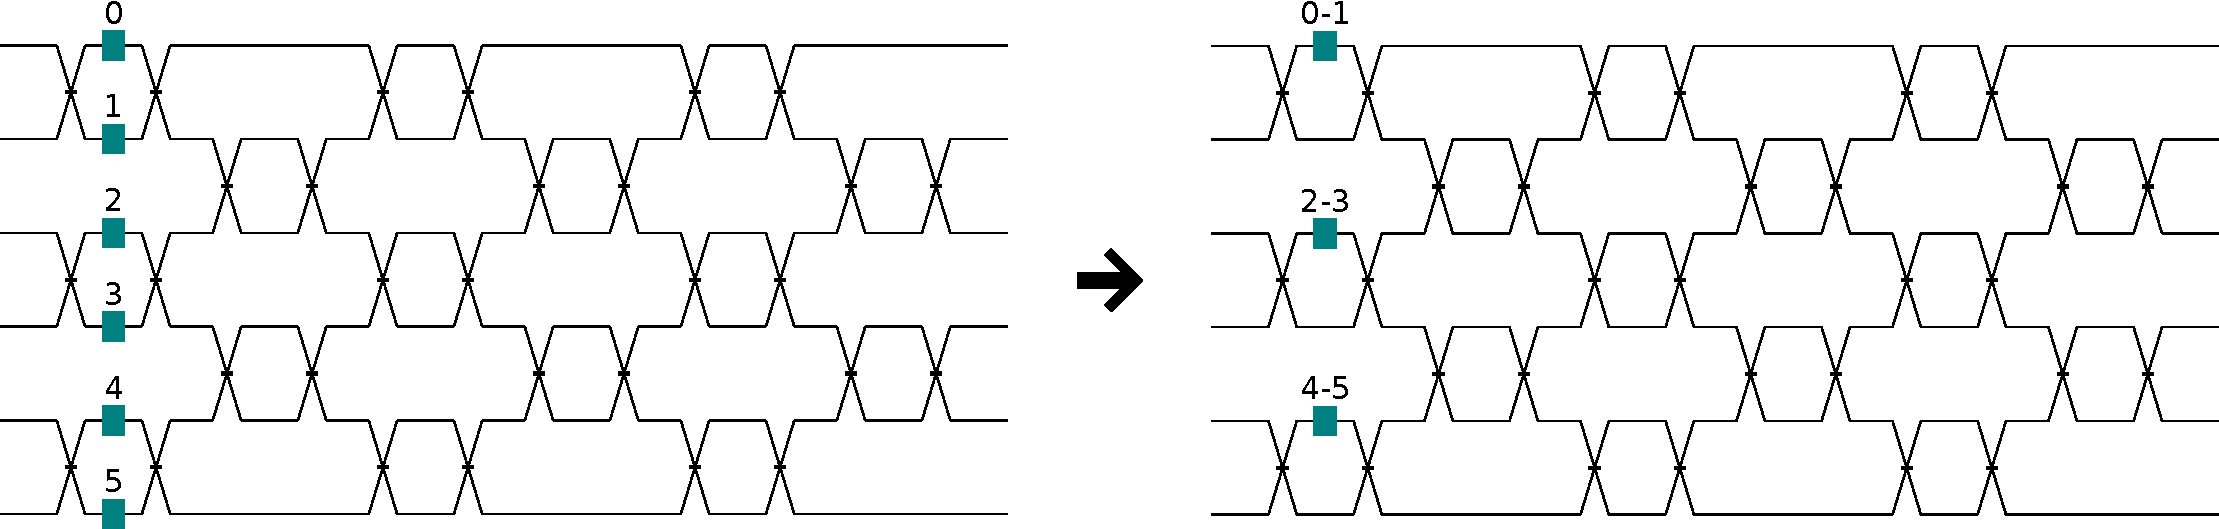
\includegraphics[width=\textwidth]{clements_xtalk_int_1.pdf} % Replace with your filename
        \caption{Column 1.} % Optional
        \label{fig:clements_xtalk_int_1}
    \end{subfigure}
    
    \vspace{0.5cm} % Vertical space between subfigures
    
    % Subfigure 2
    \begin{subfigure}{\textwidth}
        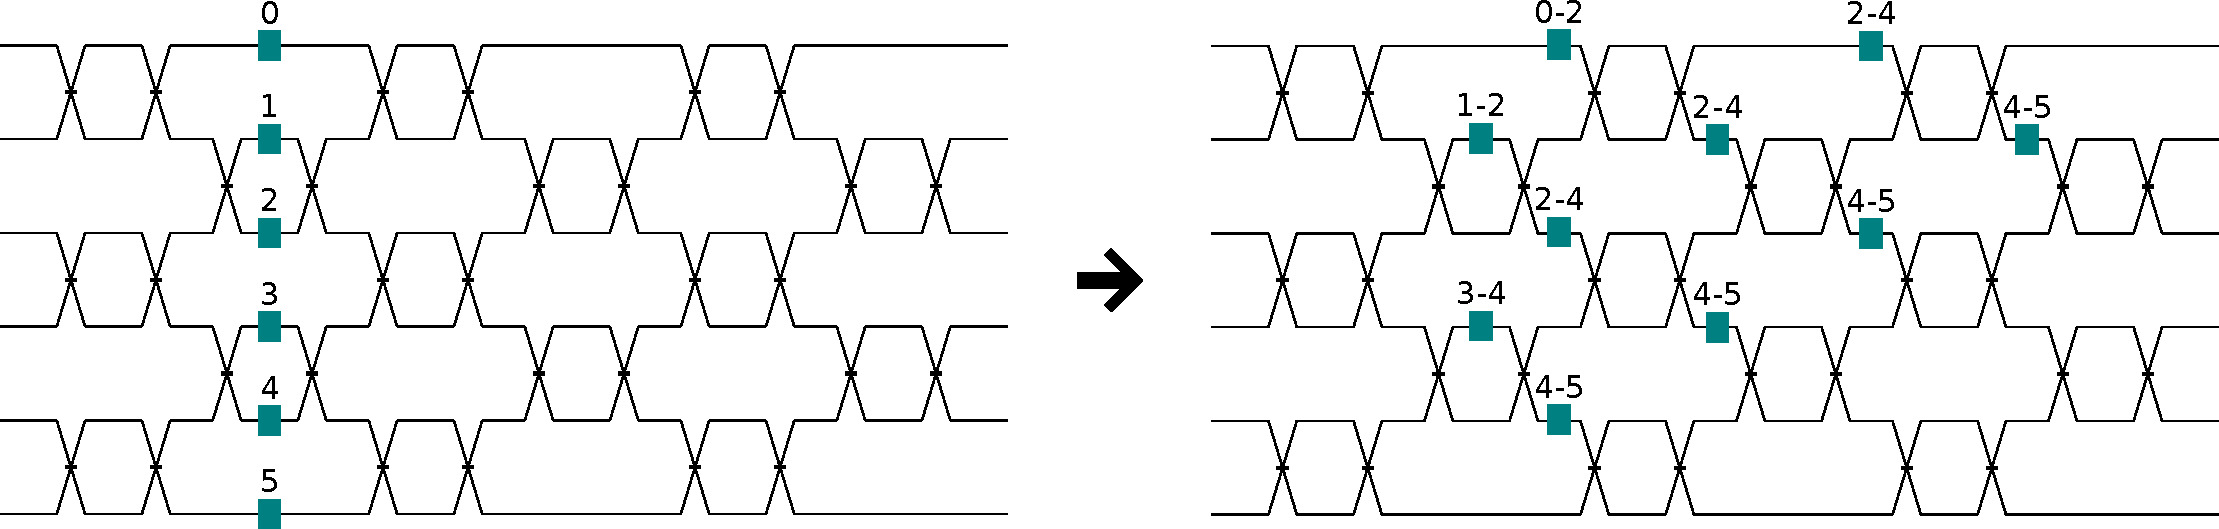
\includegraphics[width=\textwidth]{clements_xtalk_int_2.pdf}
        \caption{Column 2.}
        \label{fig:clements_xtalk_int_2}
    \end{subfigure}
    
    \vspace{0.5cm}
    
    % Subfigure 3
    \begin{subfigure}{\textwidth}
        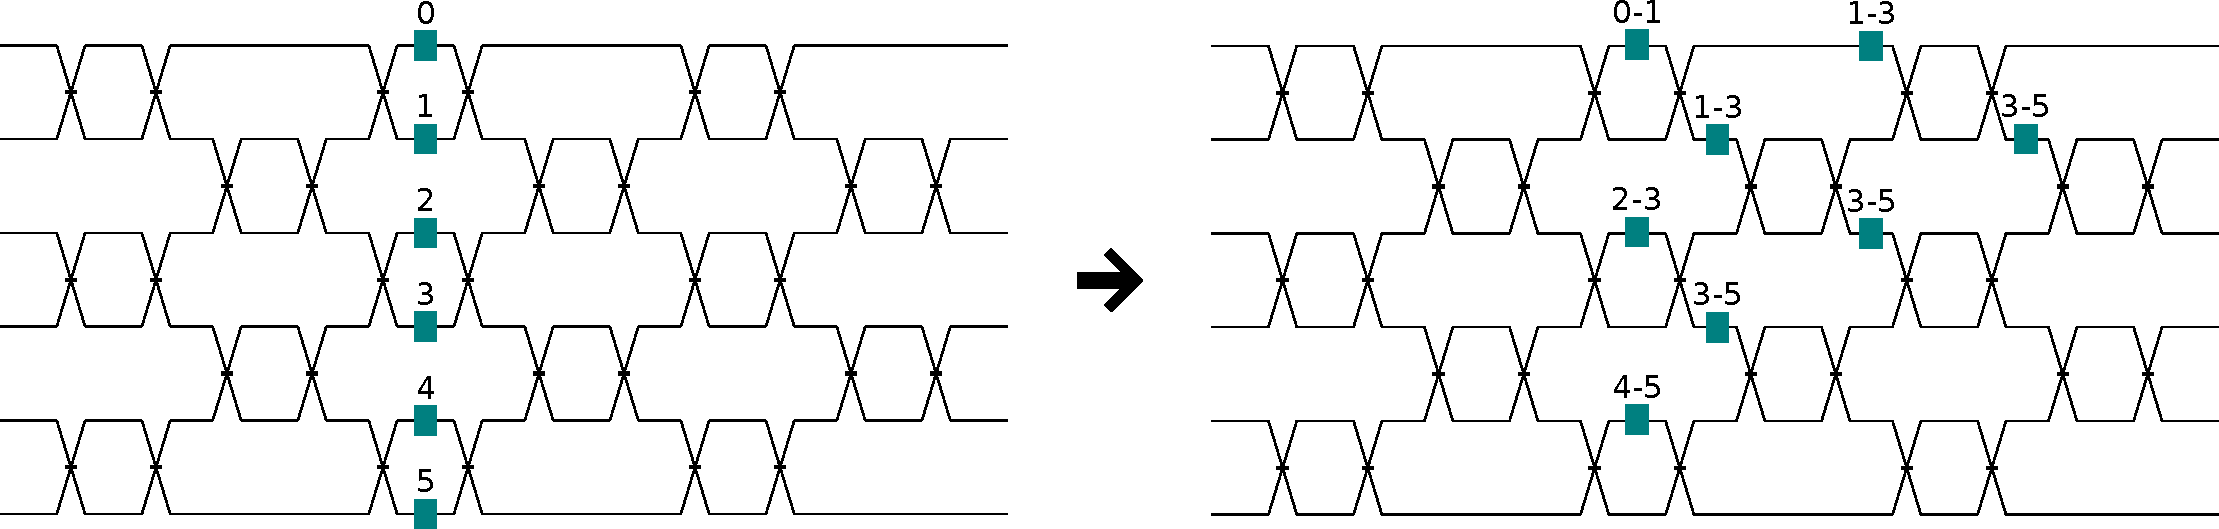
\includegraphics[width=\textwidth]{clements_xtalk_int_3.pdf}
        \caption{Column 3.}
        \label{fig:clements_xtalk_int_3}
    \end{subfigure}
    
\end{figure}

% --- NEW PAGE --- %

\begin{figure}[htbp]
    \ContinuedFloat % <--- This tells LaTeX this continues the previous figure
    \centering
    
    % Subfigure 4
    \begin{subfigure}{\textwidth}
        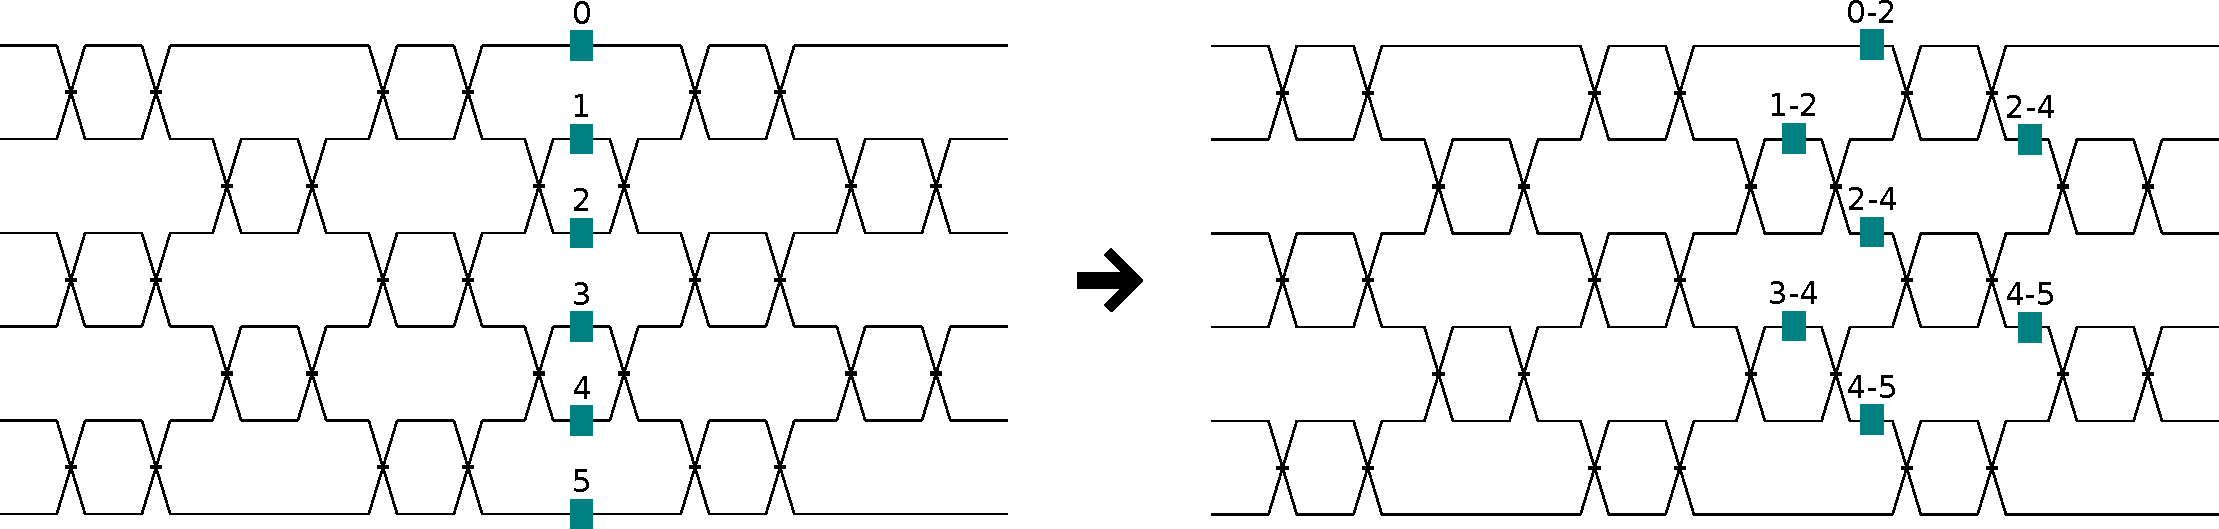
\includegraphics[width=\textwidth]{clements_xtalk_int_4.pdf}
        \caption{Column 4.}
        \label{fig:clements_xtalk_int_4}
    \end{subfigure}
    
    \vspace{0.5cm}
    
    % Subfigure 5
    \begin{subfigure}{\textwidth}
        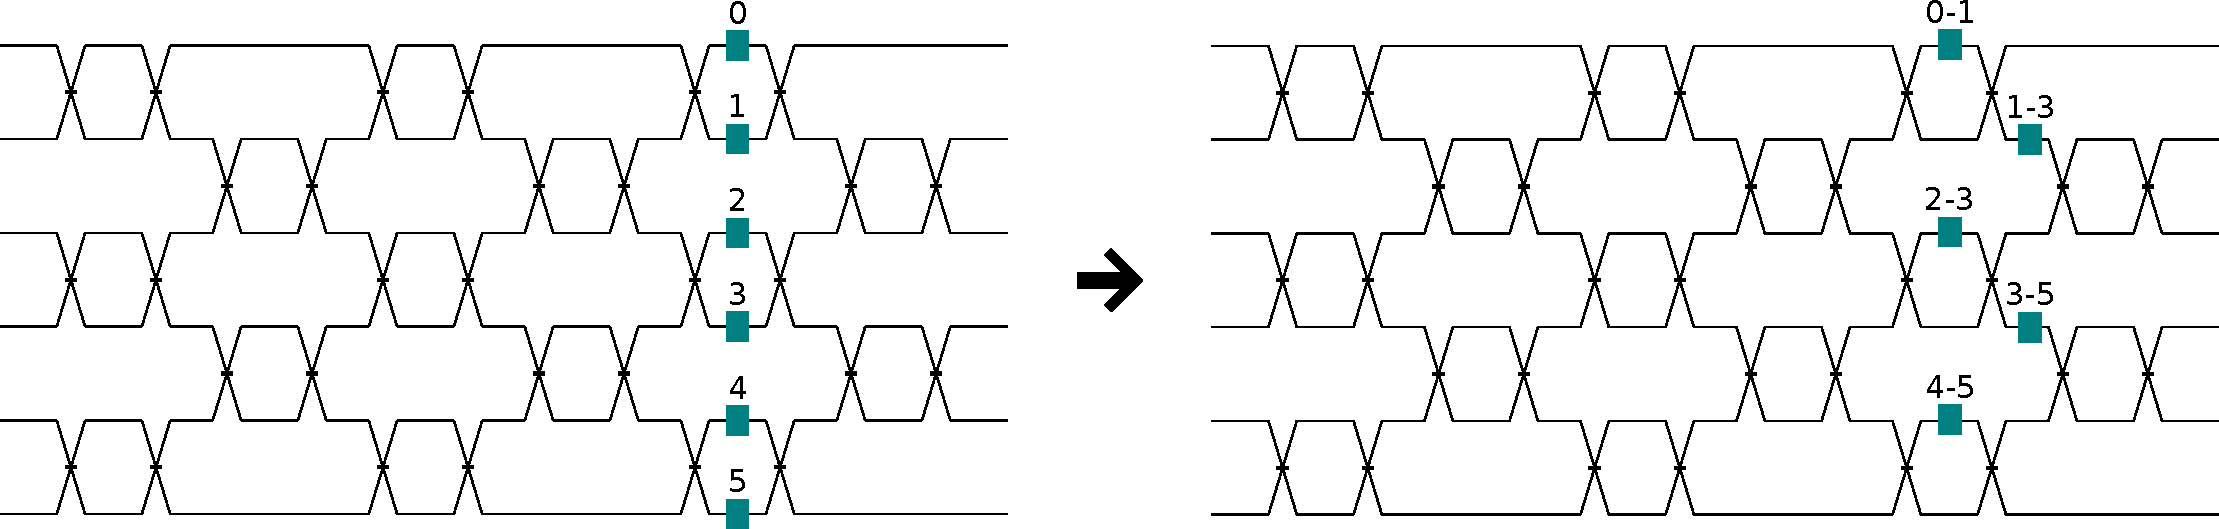
\includegraphics[width=\textwidth]{clements_xtalk_int_5.pdf}
        \caption{Column 5.}
        \label{fig:clements_xtalk_int_5}
    \end{subfigure}
    
    \vspace{0.5cm}
    
    % Subfigure 6
    \begin{subfigure}{\textwidth}
        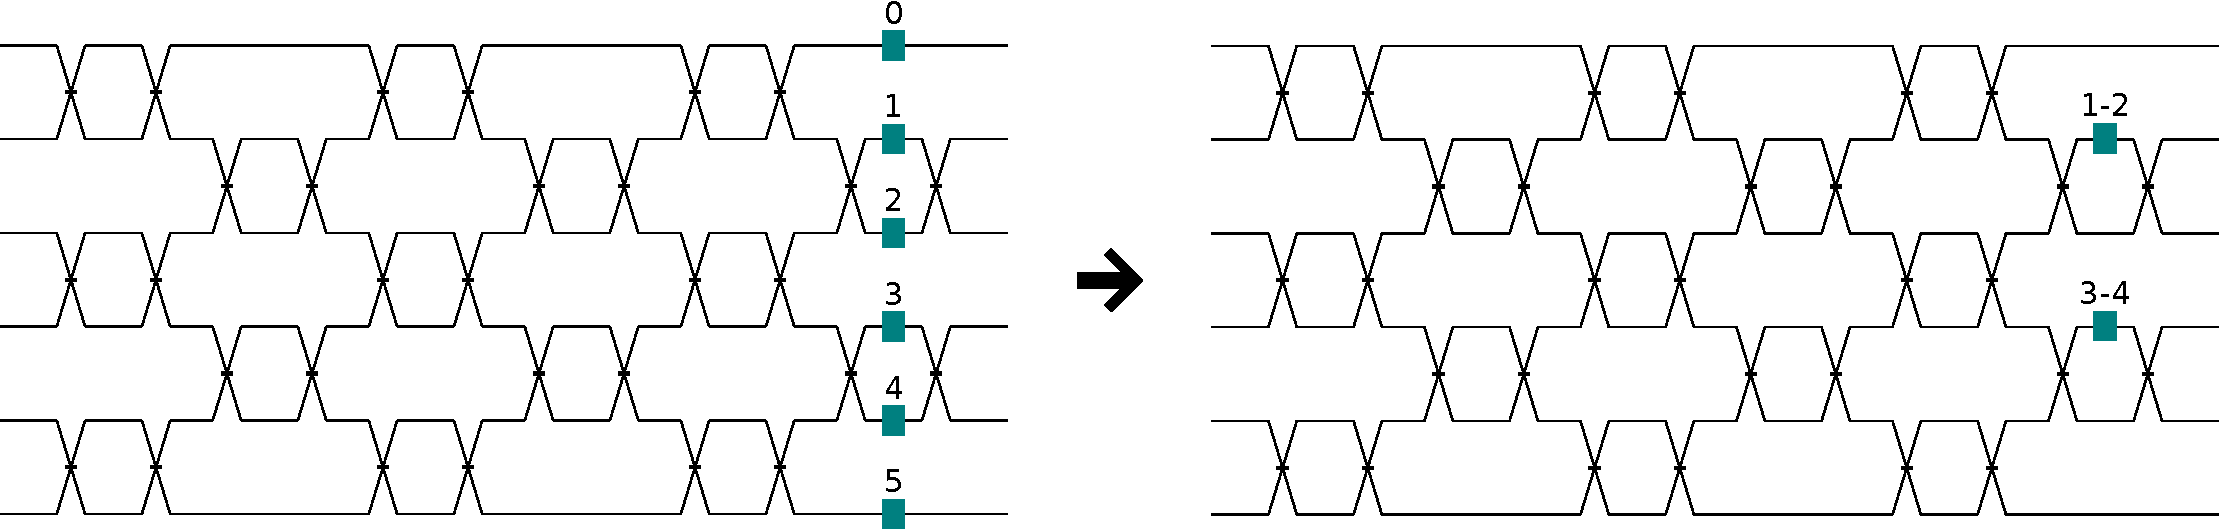
\includegraphics[width=\textwidth]{clements_xtalk_int_6.pdf}
        \caption{Column 6.}
        \label{fig:clements_xtalk_int_6}
    \end{subfigure}
    
    % This is the single main caption for the entire set of subfigures
    \caption{Remapping schemes for thermal cross-talk in a 6-mode Clements processor (internal phase shifters). For each phase shifter in a given column (left), the cross-talk is strictly vertical, but not all contributions necessarily correspond to existing phases. Therefore, we remap these contributions onto the available phases (right).}
    \label{fig:clements_xtalk_int}
    
\end{figure}

\begin{figure}[htbp]
    \centering
    % Subfigure 3
    \begin{subfigure}{\textwidth}
        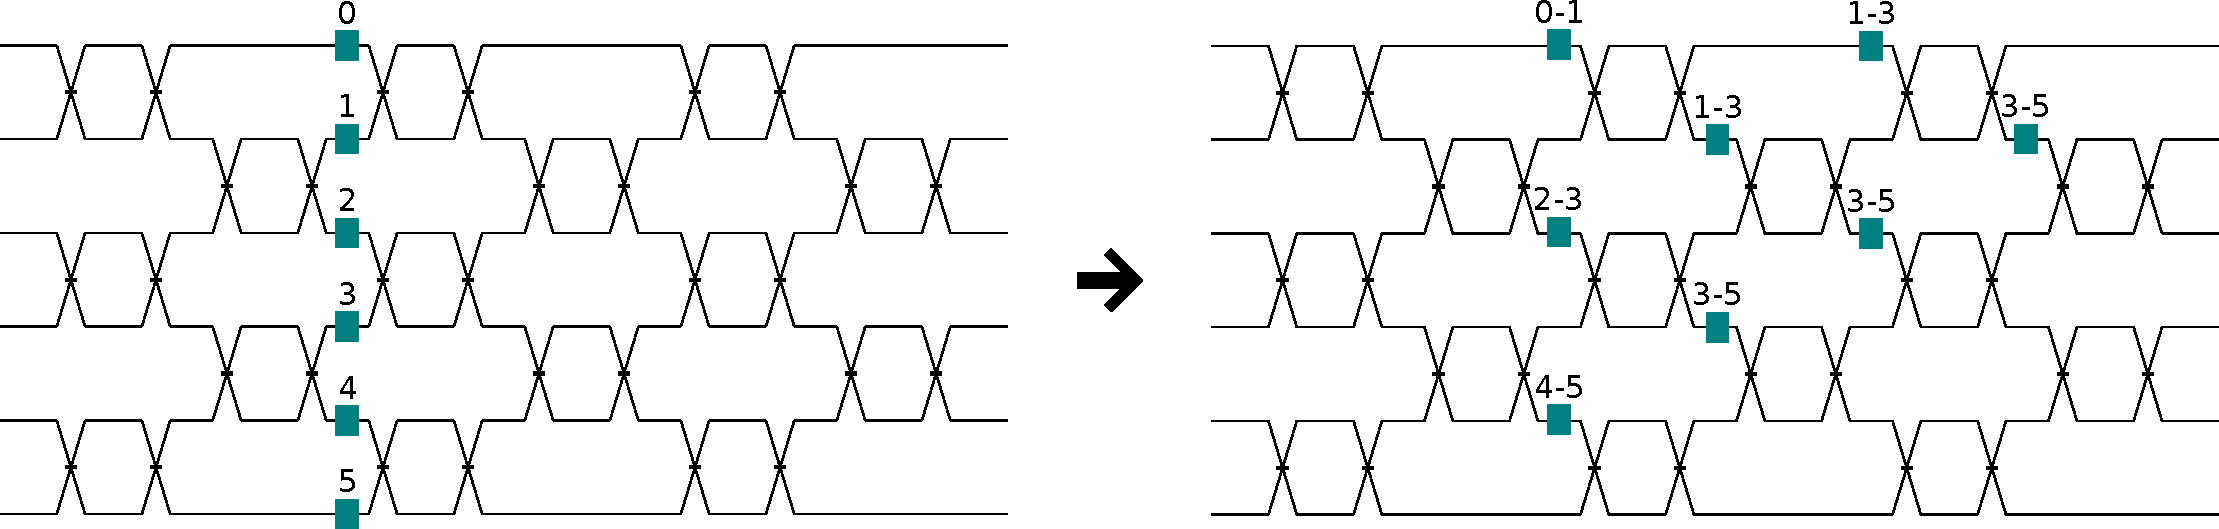
\includegraphics[width=\textwidth]{clements_xtalk_ext_3.pdf}
        \caption{Column 3.}
        \label{fig:clements_xtalk_ext_3}
    \end{subfigure}

    \vspace{0.5cm}

    % Subfigure 4
    \begin{subfigure}{\textwidth}
        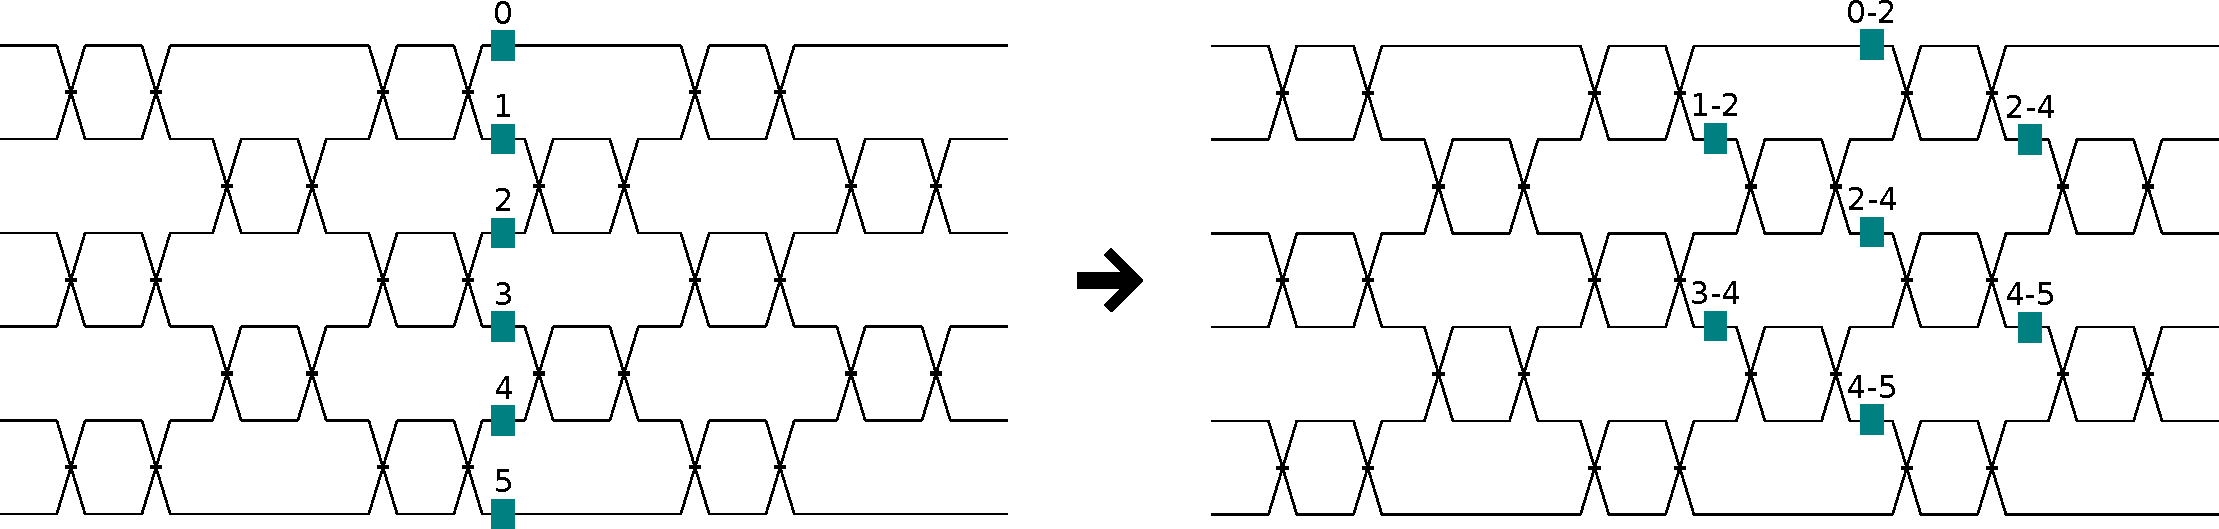
\includegraphics[width=\textwidth]{clements_xtalk_ext_4.pdf}
        \caption{Column 4.}
        \label{fig:clements_xtalk_ext_4}
    \end{subfigure}
    
    \vspace{0.5cm}
    
    % Subfigure 5
    \begin{subfigure}{\textwidth}
        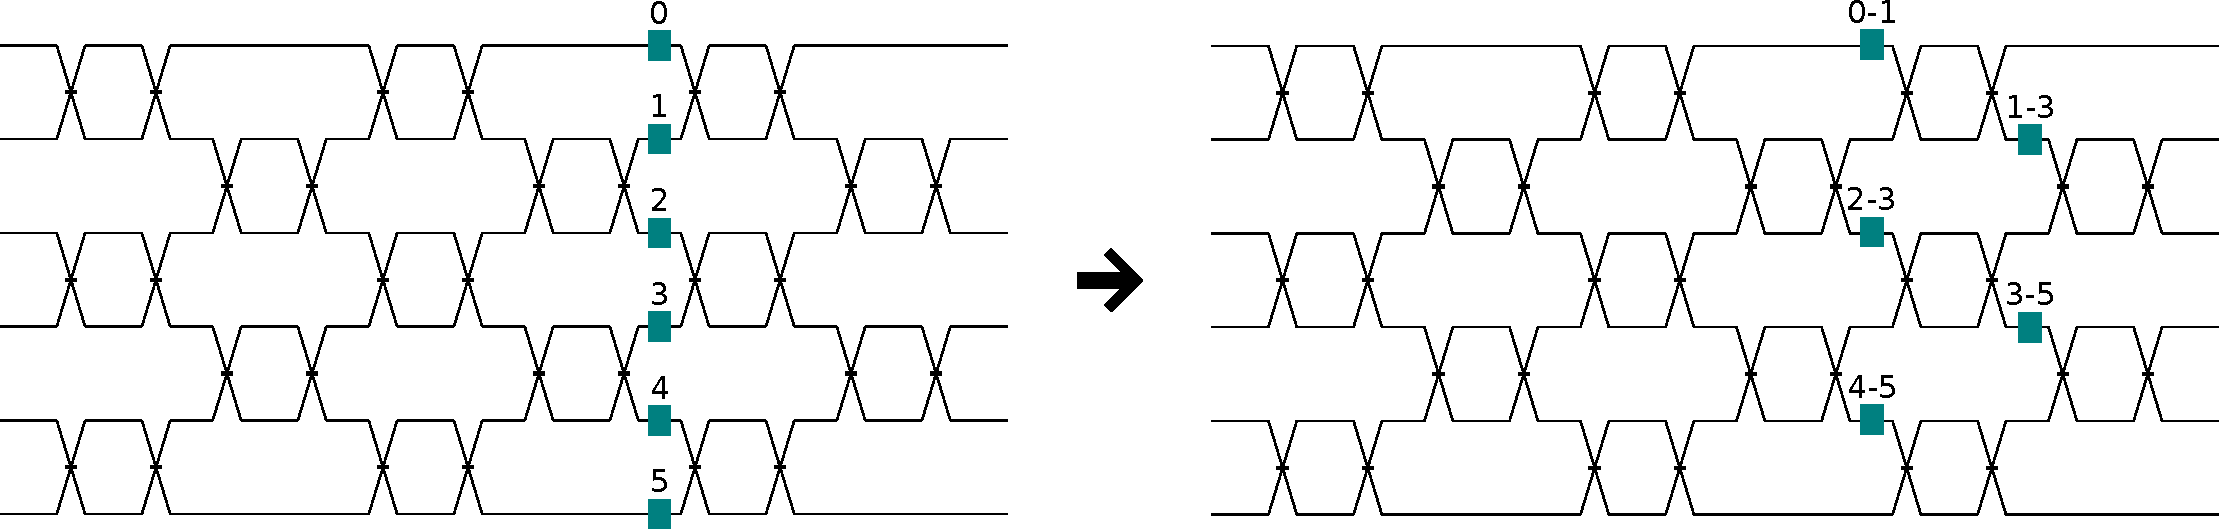
\includegraphics[width=\textwidth]{clements_xtalk_ext_5.pdf}
        \caption{Column 5.}
        \label{fig:clements_xtalk_ext_5}
    \end{subfigure}
    
    \vspace{0.5cm}

    % Subfigure 6
    \begin{subfigure}{\textwidth}
        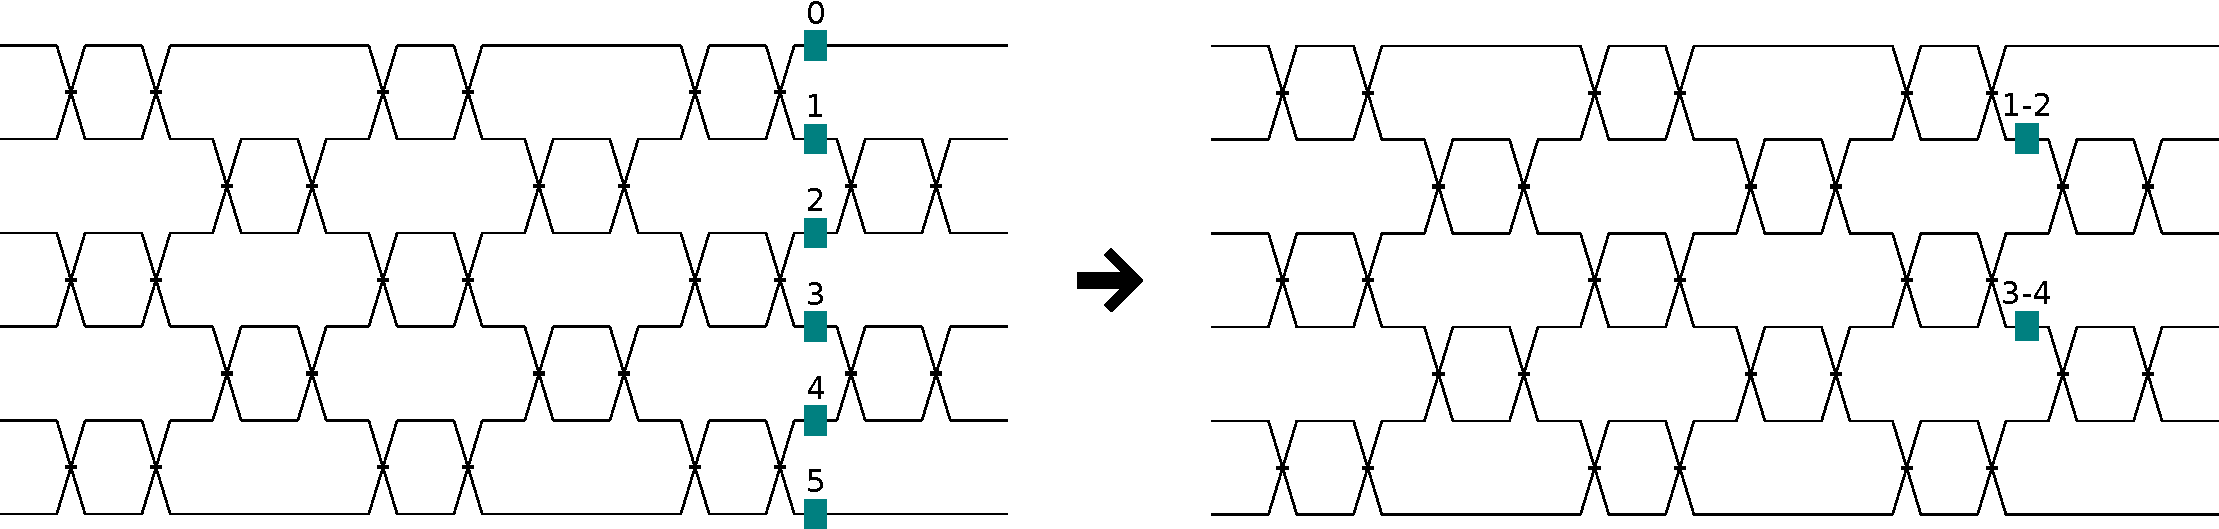
\includegraphics[width=\textwidth]{clements_xtalk_ext_6.pdf}
        \caption{Column 6.}
        \label{fig:clements_xtalk_ext_6}
    \end{subfigure}
    
    % This is the single main caption for the entire set of subfigures
    \caption{Remapping schemes for thermal cross-talk in a 6-mode Clements processor (external phase shifters). For each phase shifter in a given column (left), the cross-talk is strictly vertical, but not all contributions necessarily correspond to existing phases. Therefore, we remap these contributions onto the available phases (right). The first two columns are omitted since they do not contain active phase shifters.}
    \label{fig:clements_xtalk_ext}

\end{figure}

\section{Bell Model}
\label{sec:bell}
Figure \ref{fig:bell_base} illustrates the waveguide and phase shifter topology for a Bell UPP, based on a more compact architecture. Unlike the Clements design, this architecture compactifies the mesh by incorporating almost all phase shifters inside the MZIs (depicted in red), with only a minimal specific subset of phase shifters remaining external (in blue). The entire circuit can be viewed either as a mesh of MZI cells or, more conveniently from a computational perspective, as a cascade of alternating mixing and phase layers. While the mixing layers are shared between both the Clements and Bell architectures, the phase shifter arrangement differs; consequently, architecture-dependent methods such as \texttt{U\_from\_phases} and \texttt{phases\_from\_U} are implemented directly within the respective derived classes. Finally, Figure \ref{fig:bell_base} also details the phase shifter numbering scheme utilized in the software implementation.
\begin{figure}[htbp]
    \centering
    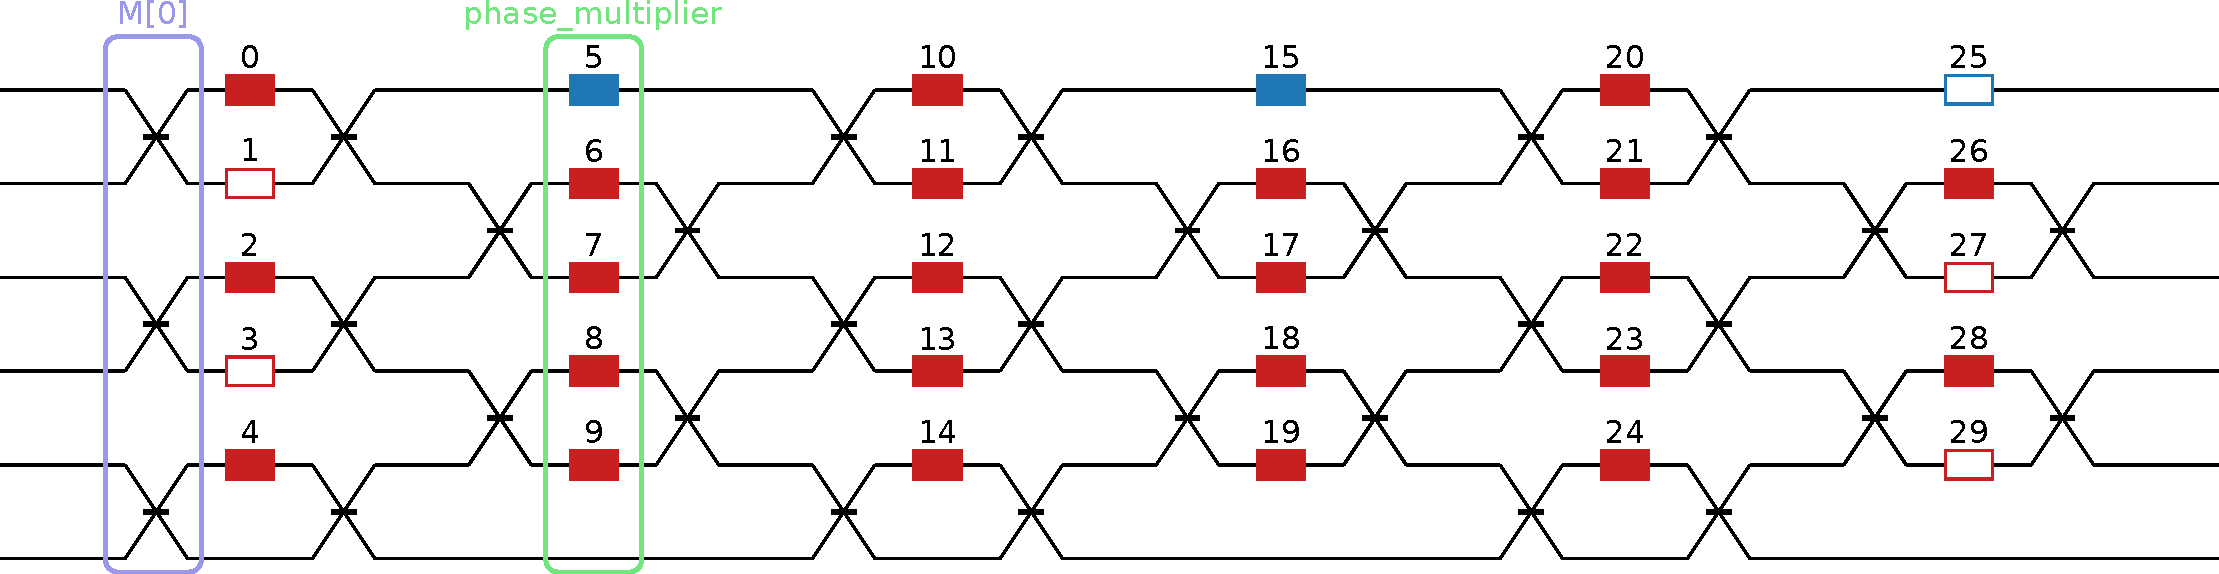
\includegraphics[width=\textwidth]{bell_base.pdf}
    \caption{Topology and numbering scheme for a 6-mode Bell processor. We highlight the first mixing layer \texttt{M[0]} and the \texttt{phase\_multiplier} variable corresponding to iteration 2.}
    \label{fig:bell_base}
\end{figure}

\subsection{Used Phases}
Figure \ref{fig:bell_base} illustrates the phase shifters actively used (depicted as solid) for circuit operation versus those considered redundant (hollow ones). This directly affects the structure of the \texttt{phases}, \texttt{currents}, and \texttt{static\_phases} vectors. Specifically, elements corresponding to redundant phase shifters are forced to zero via the \texttt{static\_phases\_mask}, following the numbering scheme shown in Figure \ref{fig:bell_base}. Similarly, the \texttt{xtalk} matrix features identically zero rows and columns for these redundant components. Examples of the \texttt{static\_phases\_mask} are provided in the accompanying spreadsheet \texttt{bell\_masking.xlsx}.

\subsection{Thermal Cross-talk}
The \texttt{xtalk} matrix exhibits a simpler structure characterized by non-zero elements concentrated around the main diagonal, an arrangement enforced by the \texttt{xtalk\_mask}. This structure arises because thermal actuation predominantly spreads heat to adjacent waveguides that already possess dedicated phase shifters, thus requiring only minimal remapping. Figure \ref{fig:bell_xtalk} illustrates these cross-talk contributions, which remain purely vertical after remapping, in contrast to the Clements architecture. Examples of the \texttt{xtalk\_mask} are provided in the accompanying spreadsheet \texttt{bell\_masking.xlsx}.
\begin{figure}[htbp]
    \centering
    % Subfigure 1
    \begin{subfigure}{\textwidth}
        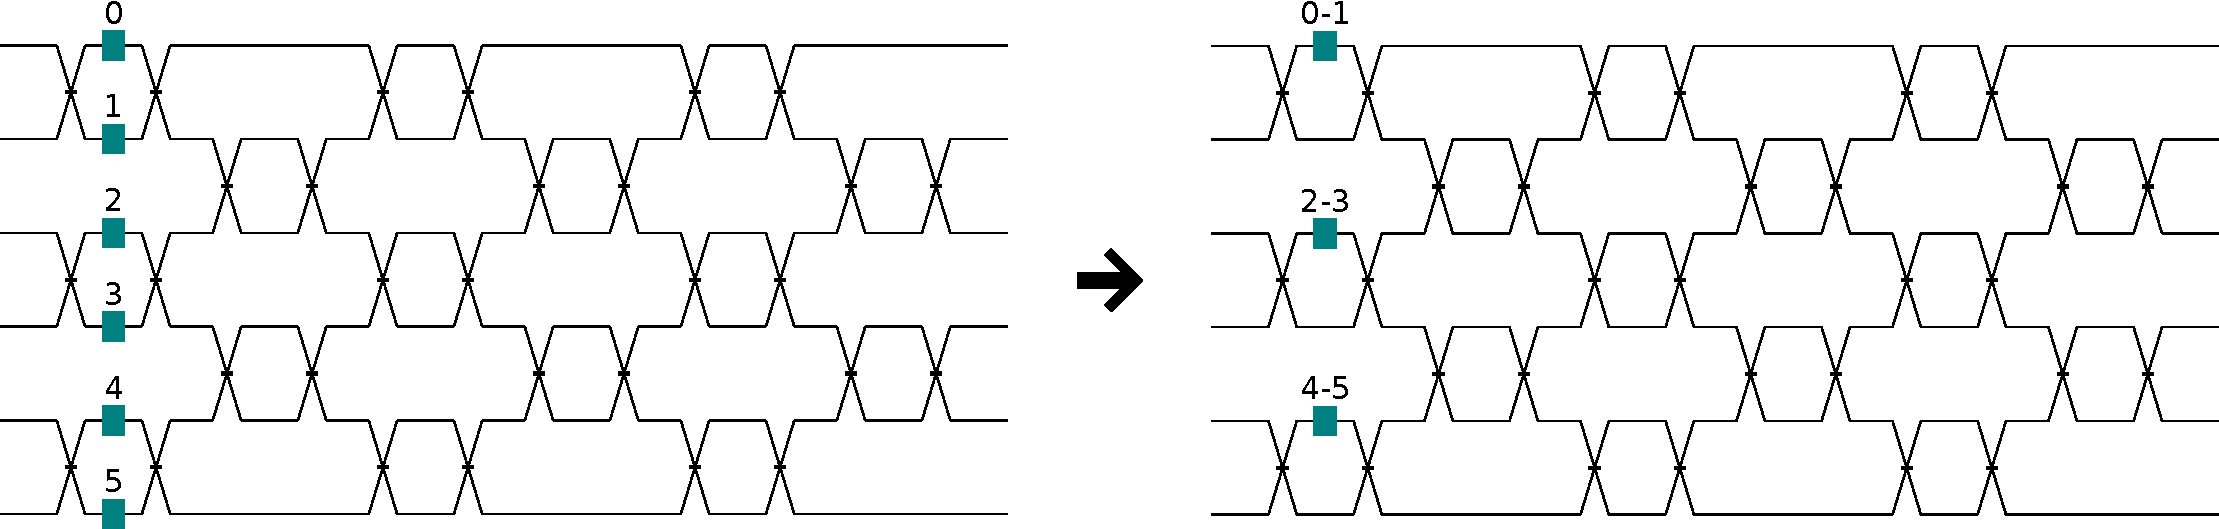
\includegraphics[width=\textwidth]{bell_xtalk_1.pdf}
        \caption{Column 1.}
        \label{fig:bell_xtalk_1}
    \end{subfigure}
    
    \vspace{0.5cm} % Vertical space between subfigures
    
    % Subfigure 2
    \begin{subfigure}{\textwidth}
        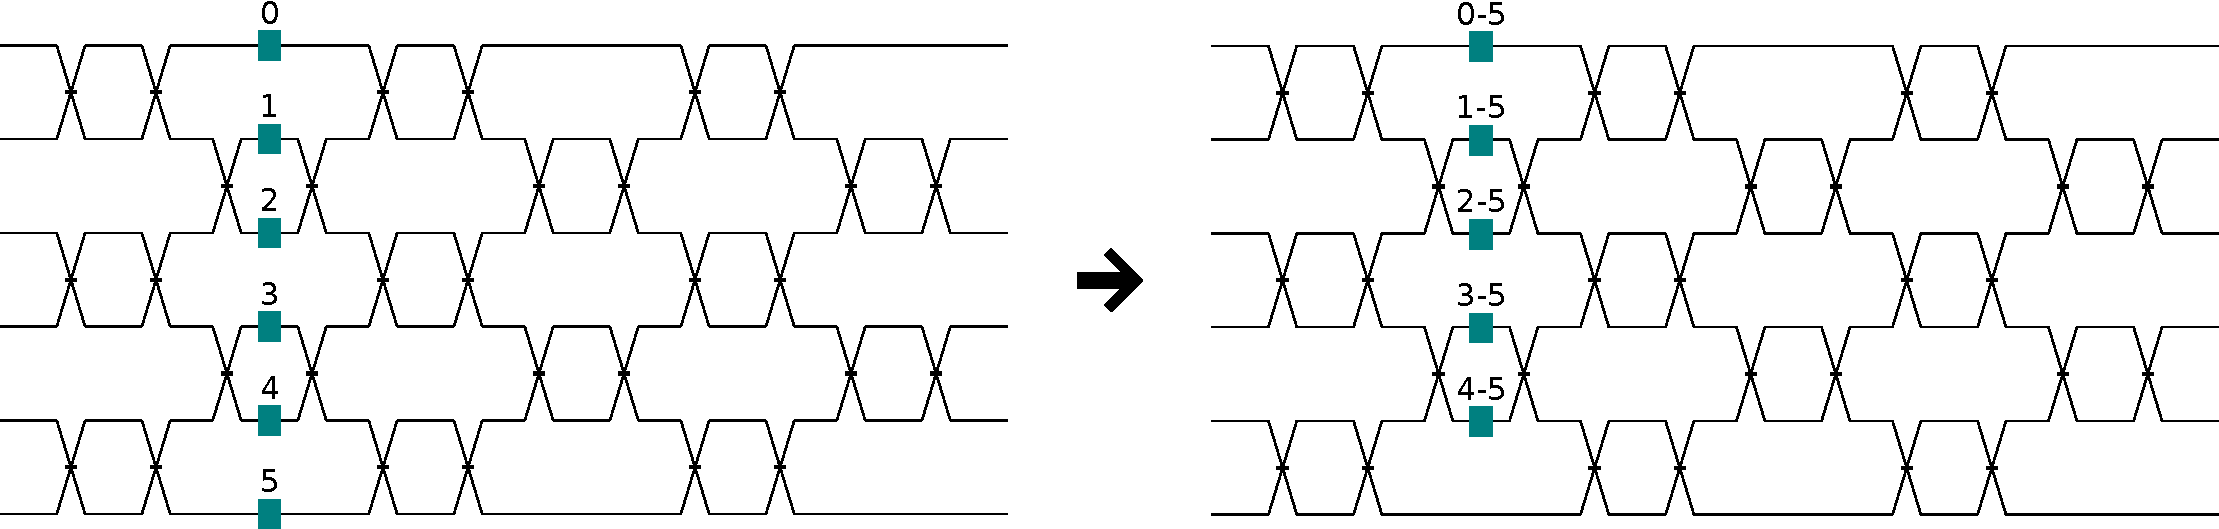
\includegraphics[width=\textwidth]{bell_xtalk_2.pdf}
        \caption{Column 2.}
        \label{fig:bell_xtalk_2}
    \end{subfigure}

    \vspace{0.5cm}

    % Subfigure 3
    \begin{subfigure}{\textwidth}
        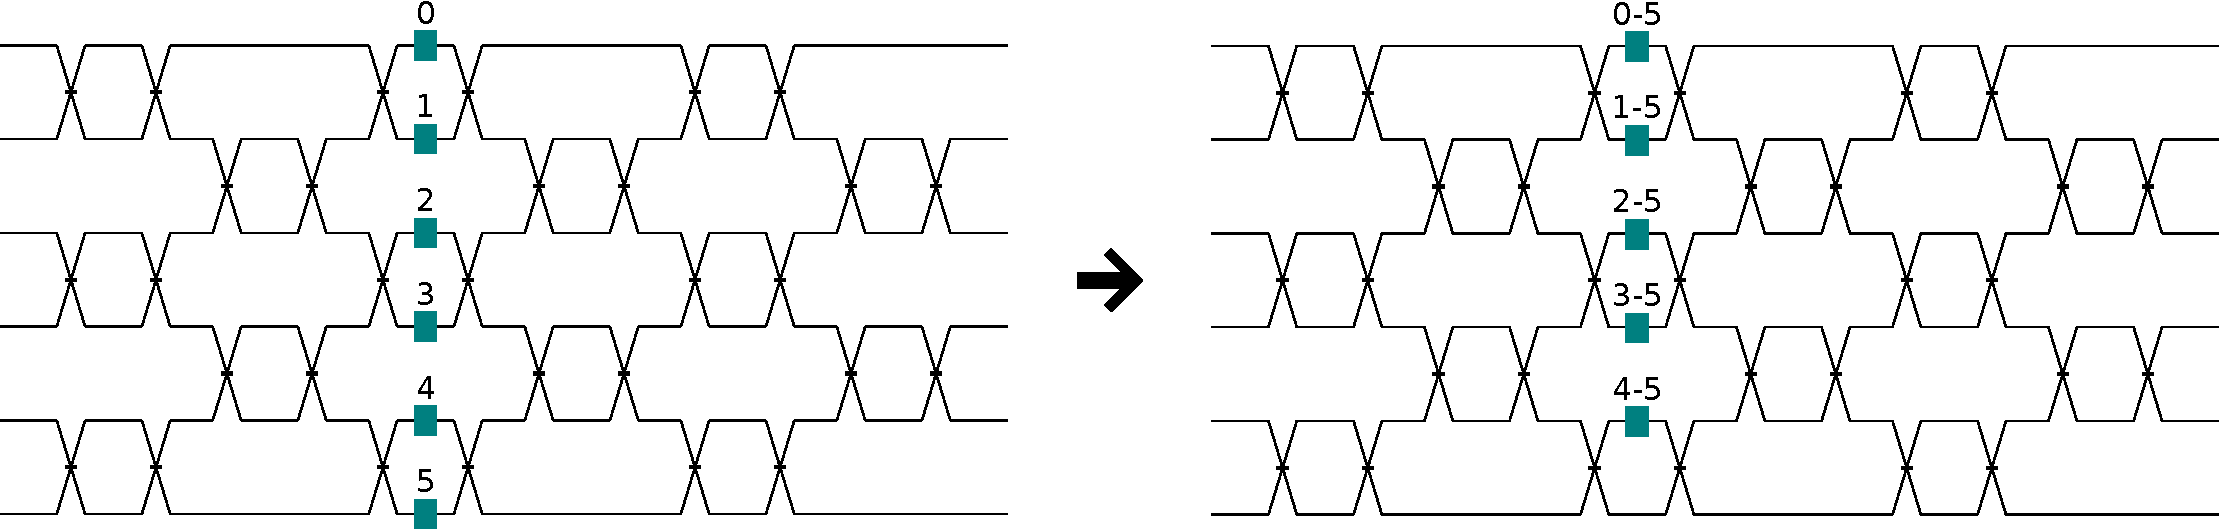
\includegraphics[width=\textwidth]{bell_xtalk_3.pdf}
        \caption{Column 3.}
        \label{fig:bell_xtalk_3}
    \end{subfigure}

    \vspace{0.5cm}

    % Subfigure 4
    \begin{subfigure}{\textwidth}
        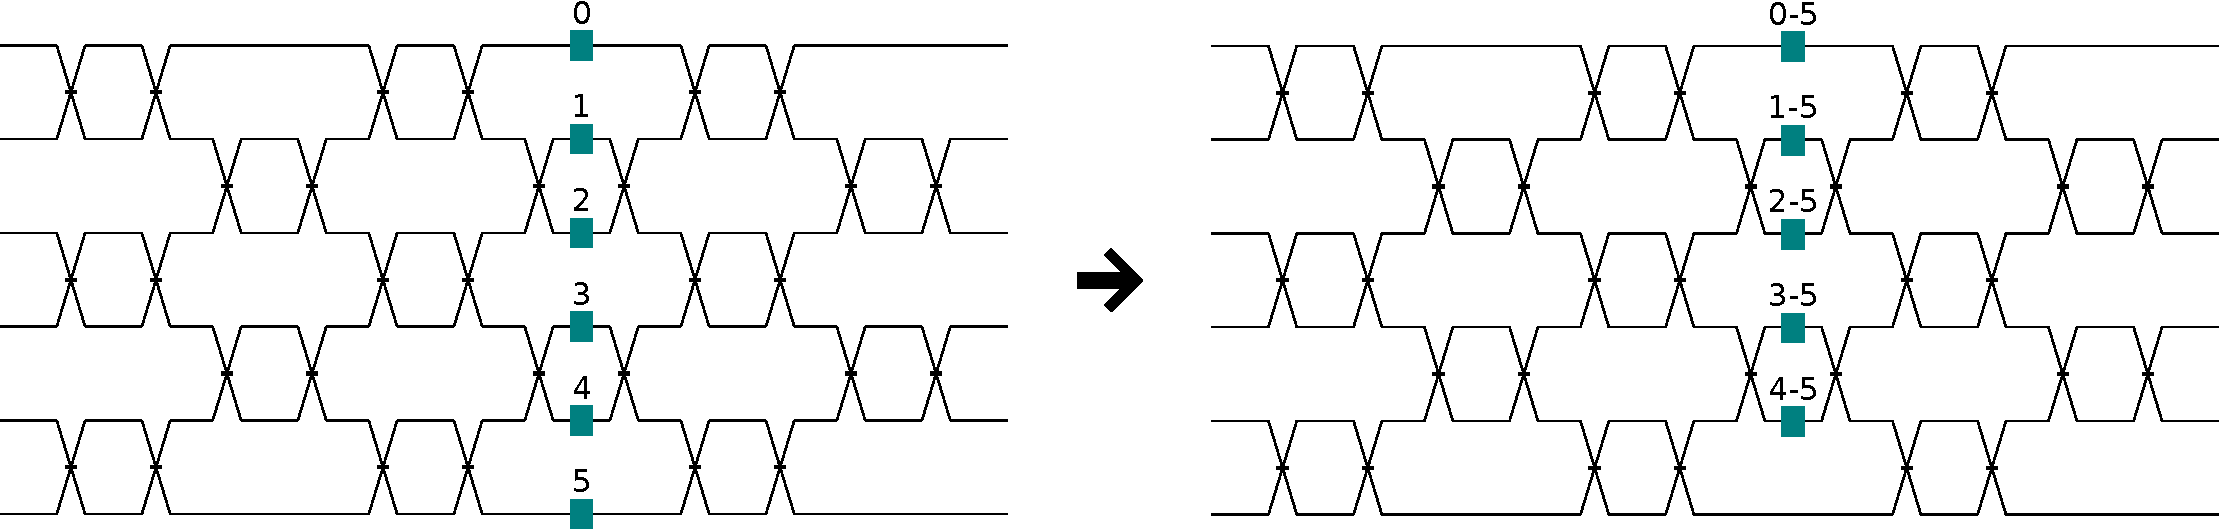
\includegraphics[width=\textwidth]{bell_xtalk_4.pdf}
        \caption{Column 4.}
        \label{fig:bell_xtalk_4}
    \end{subfigure}

\end{figure}

% --- NEW PAGE --- %

\begin{figure}[htbp]
    \ContinuedFloat % <--- This tells LaTeX this continues the previous figure
    \centering
        
    % Subfigure 5
    \begin{subfigure}{\textwidth}
        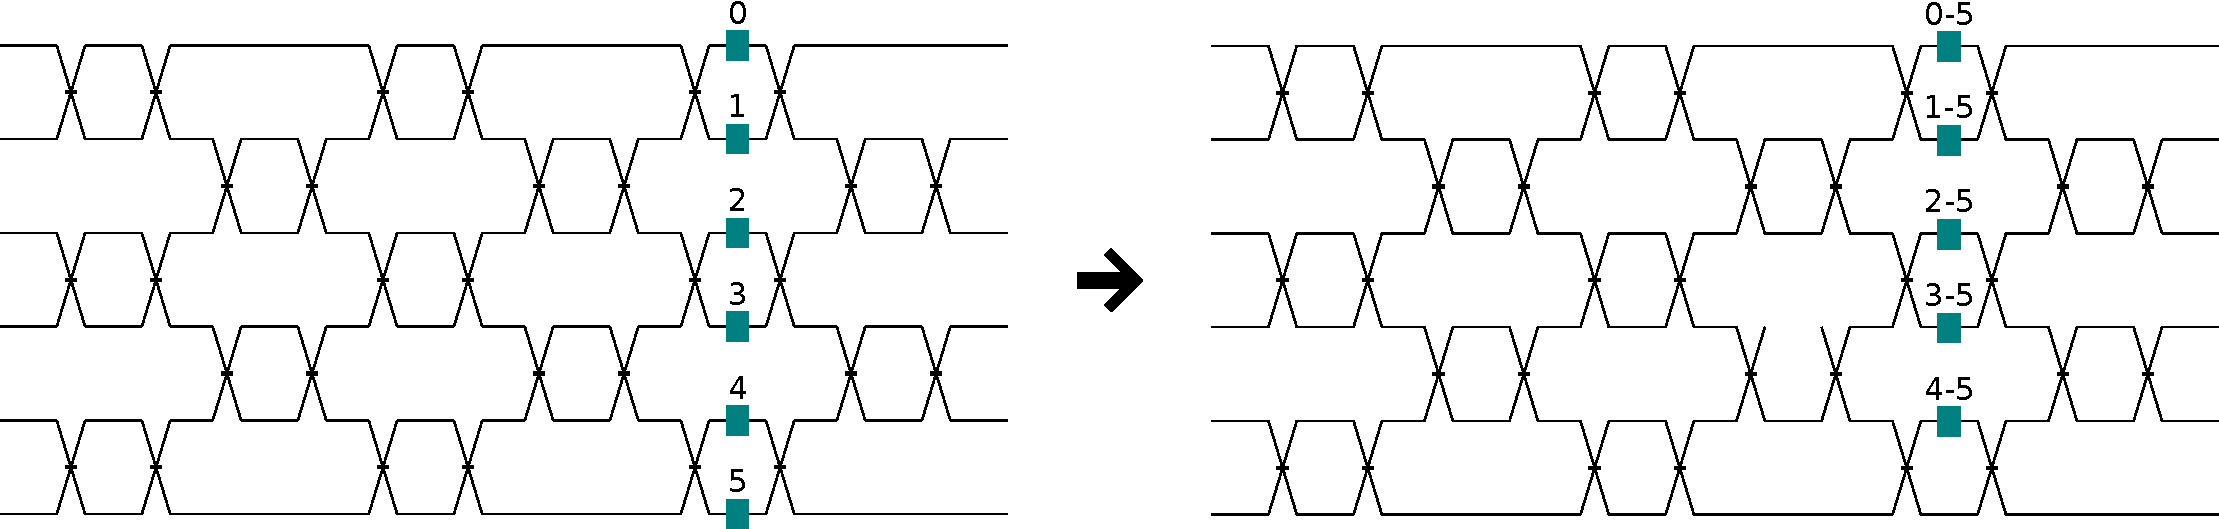
\includegraphics[width=\textwidth]{bell_xtalk_5.pdf}
        \caption{Column 5.}
        \label{fig:bell_xtalk_5}
    \end{subfigure}
    
    \vspace{0.5cm}
    
    % Subfigure 6
    \begin{subfigure}{\textwidth}
        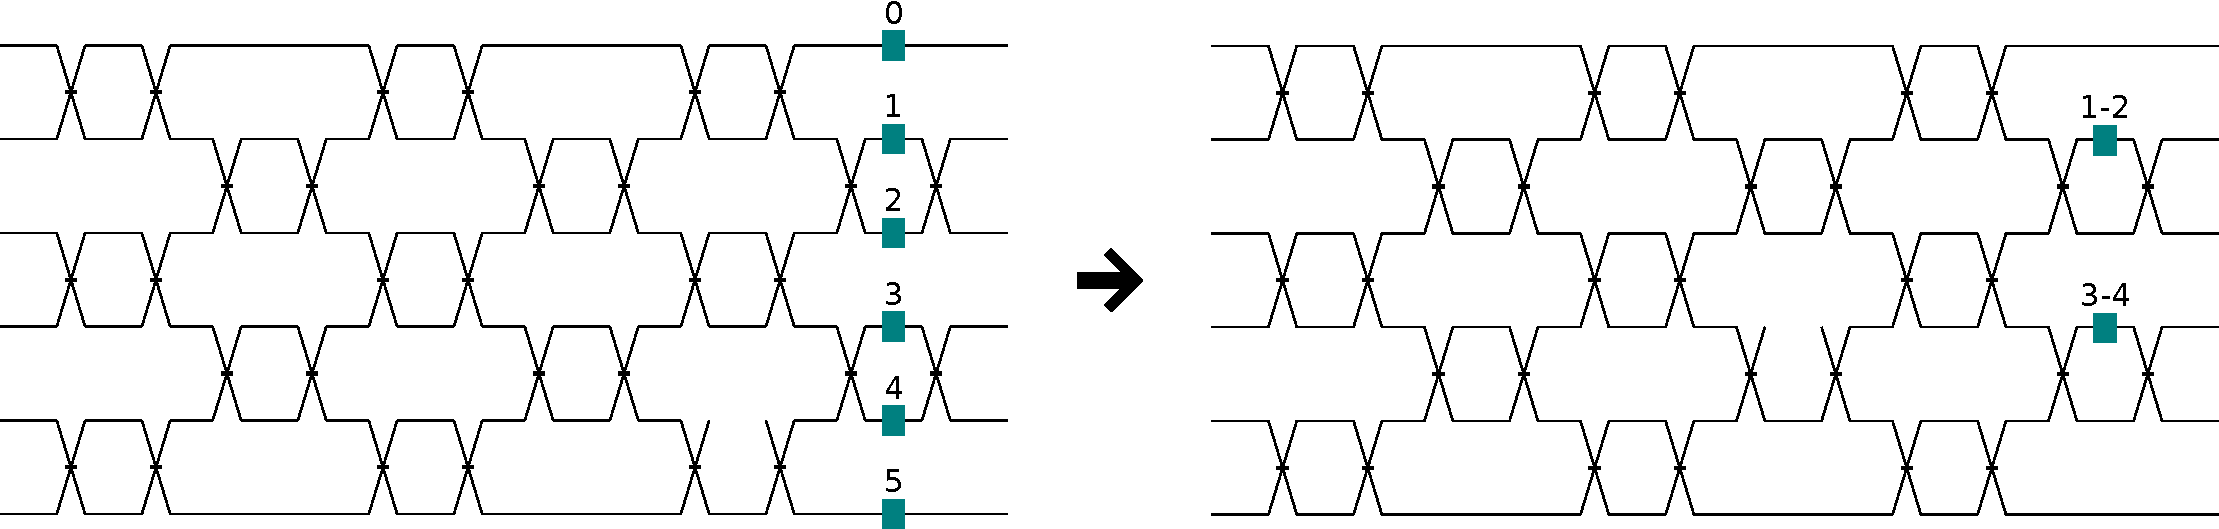
\includegraphics[width=\textwidth]{bell_xtalk_6.pdf}
        \caption{Column 6.}
        \label{fig:bell_xtalk_6}
    \end{subfigure}
    
    % This is the single main caption for the entire set of subfigures
    \caption{Remapping schemes for thermal cross-talk in a 6-mode Bell processor. For each phase shifter in a given column (left), the cross-talk is strictly vertical, but not all contributions necessarily correspond to existing phases. Therefore, we remap these contributions onto the available phases (right).}
    \label{fig:bell_xtalk}
    
\end{figure}

\end{document}
